
\documentclass{standalone}

\usepackage{tikz}
\usetikzlibrary{calc}
\usetikzlibrary{math} % for \tikzmath
\usetikzlibrary{angles,quotes} % for pic (angle labels)
\begin{document}
% TANGENT to CIRCLE - known: r, alpha
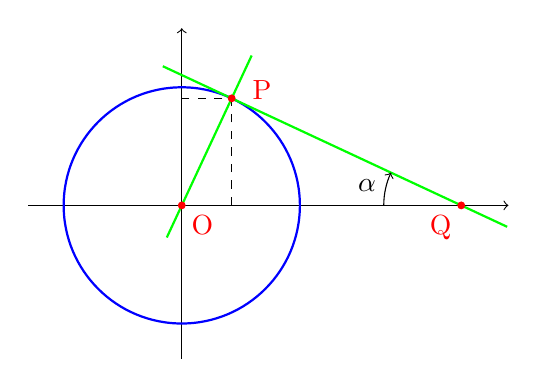
\begin{tikzpicture}
  \def\r{1.5} % radius
  \def\ang{25} % alpha angle
  \def\q{\r/sin(\ang)} % distance center-external point q = |OQ|
  \coordinate (O) at (0,0); % circle center O
  \coordinate (Q) at ({\q},0); % external point Q
  \coordinate (P) at (90-\ang:\r); % point of tangency, P
  \draw[->] (0,-1.3*\r) -- (0,1.5*\r);
  \draw[->] (-1.3*\r,0) -- ({\q+0.4*\r},0);
  \draw[dashed] ({\r*sin(\ang)},0) |- (0,{\r*cos(\ang)});
  \draw[blue,thick] (O) circle(\r);
  \draw[green,thick] ($(Q)!-0.2!(P)$) -- ($(Q)!1.3!(P)$);
  \draw[green,thick] ($(O)!-0.3!(P)$) -- ($(O)!1.4!(P)$);
  \fill[red] (O) circle(0.05) node[below right] {O};
  \fill[red] (Q) circle(0.05) node[below left] {Q};
  \fill[red] (P) circle(0.05) node[above=3,right=4] {P};
  \draw pic[<-,"$\alpha$"{above=1,left=0},draw=black,angle radius=28,angle eccentricity=1.0]
    {angle = P--Q--O};
\end{tikzpicture}

% TANGENT to ELLIPSE - known: a, b, alpha
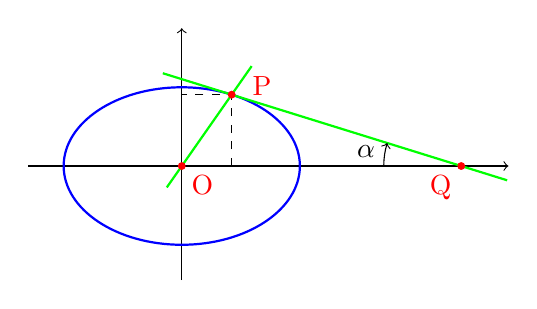
\begin{tikzpicture}
  \def\a{1.5} % horizontal radius
  \def\b{1.0} % vertical radius
  \def\ang{25} % alpha angle
  \def\q{\a/sin(\ang)} % distance center-external point q = |OQ|
  \coordinate (O) at (0,0); % circle center O
  \coordinate (Q) at ({\q},0); % external point Q
  \coordinate (P) at (90-\ang:{\a} and {\b}); % point of tangency, P
  \draw[->] (0,-\b-0.3*\a) -- (0,\b+0.5*\a);
  \draw[->] (-1.3*\a,0) -- ({\q+0.4*\a},0);
  \draw[dashed] ({\a*sin(\ang)},0) |- (0,{\b*cos(\ang)});
  \draw[blue,thick] (O) ellipse({\a} and {\b});
  \draw[green,thick] ($(Q)!-0.2!(P)$) -- ($(Q)!1.3!(P)$);
  \draw[green,thick] ($(O)!-0.3!(P)$) -- ($(O)!1.4!(P)$);
  \fill[red] (O) circle(0.05) node[below right] {O};
  \fill[red] (Q) circle(0.05) node[below left] {Q};
  \fill[red] (P) circle(0.05) node[above=3,right=4] {P};
  \draw pic[<-,"$\alpha$"{above=1,left=0},draw=black,angle radius=28,angle eccentricity=1.0]
    {angle = P--Q--O};
\end{tikzpicture}
\end{document}








